\documentclass[10pt, t]{beamer}
\usetheme{metropolis}           % Use metropolis theme

\ifnotes
  \hypersetup{final}
  \usepackage{pgfpages}
  \setbeamertemplate{note page}[plain]
  \setbeameroption{show notes on second screen=right}
  % the following fixes bug which causes normal text to be white instead of
  % template default when notes are enabled
  % (see https://tex.stackexchange.com/questions/232168/normal-text-is-invisible-when-using-beamer-with-notes-and-xelatex)
  \makeatletter 
  \def\beamer@framenotesbegin{% at beginning of slide
       \usebeamercolor[fg]{normal text}
        \gdef\beamer@noteitems{}% 
        \gdef\beamer@notes{}% 
  }
  \makeatother
\fi

\usepackage{appendixnumberbeamer}
\usepackage{multirow}
\usepackage{verbatim}
\usepackage{tikz}
\usetikzlibrary{decorations.pathreplacing}
\usepackage[scale=3]{ccicons}   % creative commons icons

\title{Performance analysis}
\date{}
\author{Jeremy Iverson}
\institute{College of Saint Benedict \& Saint John's University}

\begin{document}

  \begin{frame}
    \titlepage
  \end{frame}

  \begin{frame}{Performance analysis}
    \begin{itemize}
      \item how do we reason about parallel algorithms?
      \item how can we compare two algorithms and determine which is better?
      \item how do we measure improvement?
    \end{itemize}
  \end{frame}

  \begin{frame}{Performance metrics}
    \begin{itemize}
      \item execution time ($T_p$)
      \item speedup  ($S$)
      \item efficiency ($E$)
      \item cost ($C$)
    \end{itemize}
  \end{frame}

  \begin{frame}{Execution time}
    \begin{block}{Serial ($T_s$)}
      \begin{itemize}
        \item time elapsed between beginning and end of execution
      \end{itemize}
    \end{block}

    \begin{block}{Parallel ($T_p$)}
      \begin{itemize}
        \item time elapsed between beginning of execution and the moment the
          last processing element finishes execution
      \end{itemize}
    \end{block}

    \begin{itemize}
      \item Adding numbers
      \item Dot-product
      \item Matrix-vector multiplication
      \item Matrix-matrix multiplication
    \end{itemize}

    \note[item] {Adding numbers --- $T_s=\theta(n)$ --- $T_p=\theta(\log n)$}
    \note[item] {Matrix-vector --- $T_s=\theta(n^2)$ --- $T_p=\theta(n)$}
    \note[item] {Matrix-matrix --- $T_s=\theta(n^3)$ --- $T_p=\theta(n^2)$}
    \note[item] {So how long to compute mat-mat for a $10000\times10000$ mat?}
  \end{frame}

  \begin{frame}{Execution time}
    \vspace{-6ex}
    \begin{center}
      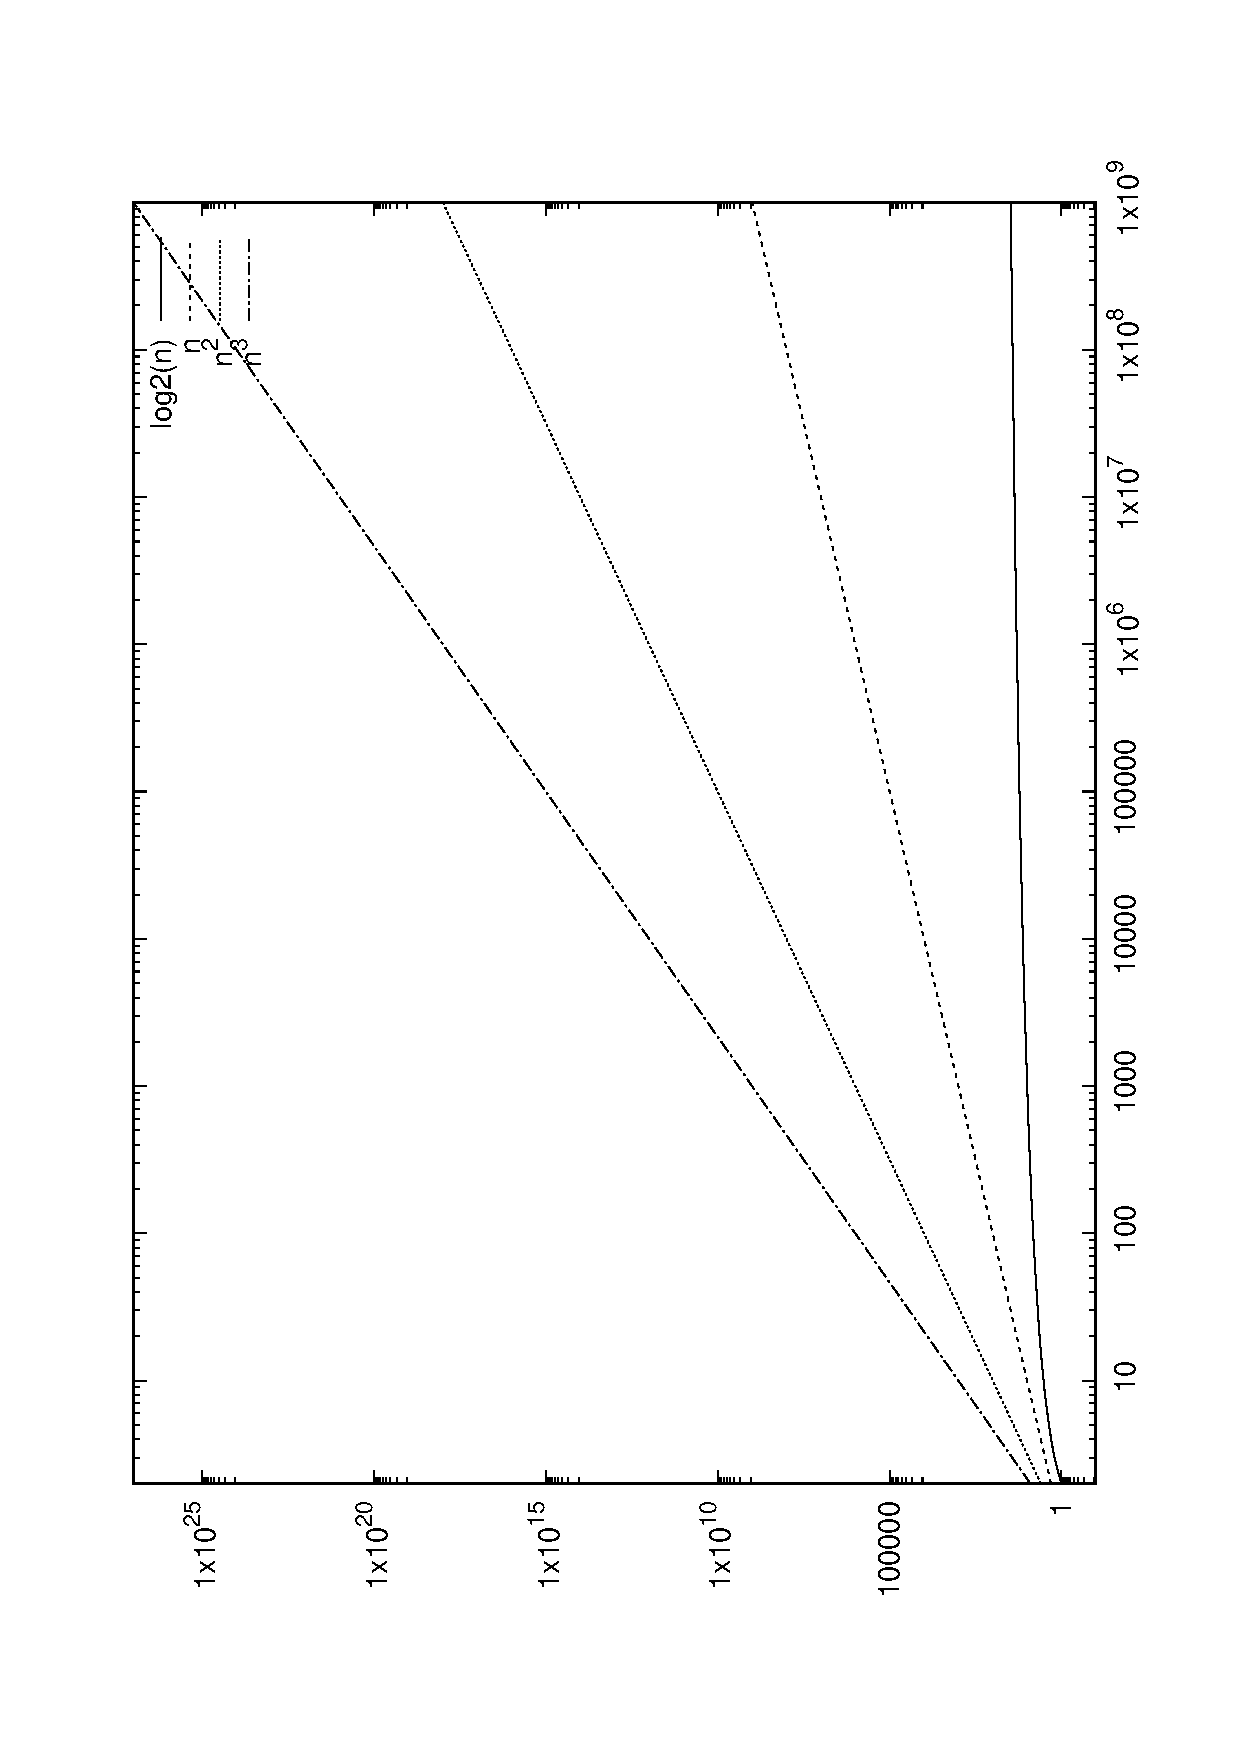
\includegraphics[width=.70\textwidth,angle=-90]{execution-time}
    \end{center}
  \end{frame}

  \begin{frame}{Speedup}
    \begin{block}{Speedup ($S=T_s/T_p$)}
      \begin{itemize}
        \item the ratio of time taken to solve a problem on a single processing
          element to the time required to solve the same problem on a parallel
          computer with $p$ processing elements
      \end{itemize}
    \end{block}
    \note[item] {Adding numbers --- $S=\theta(n/\log n)$}
    \note[item] {Matrix-vector --- $S=\theta(n^2/n)=\theta(n)$}
    \note[item] {Matrix-matrix --- $S=\theta(n^3/n^2)=\theta(n)$}
    \note[item] {What are the limits of speedup?}

    \vspace{-2ex}
    \begin{center}
      \only<2>{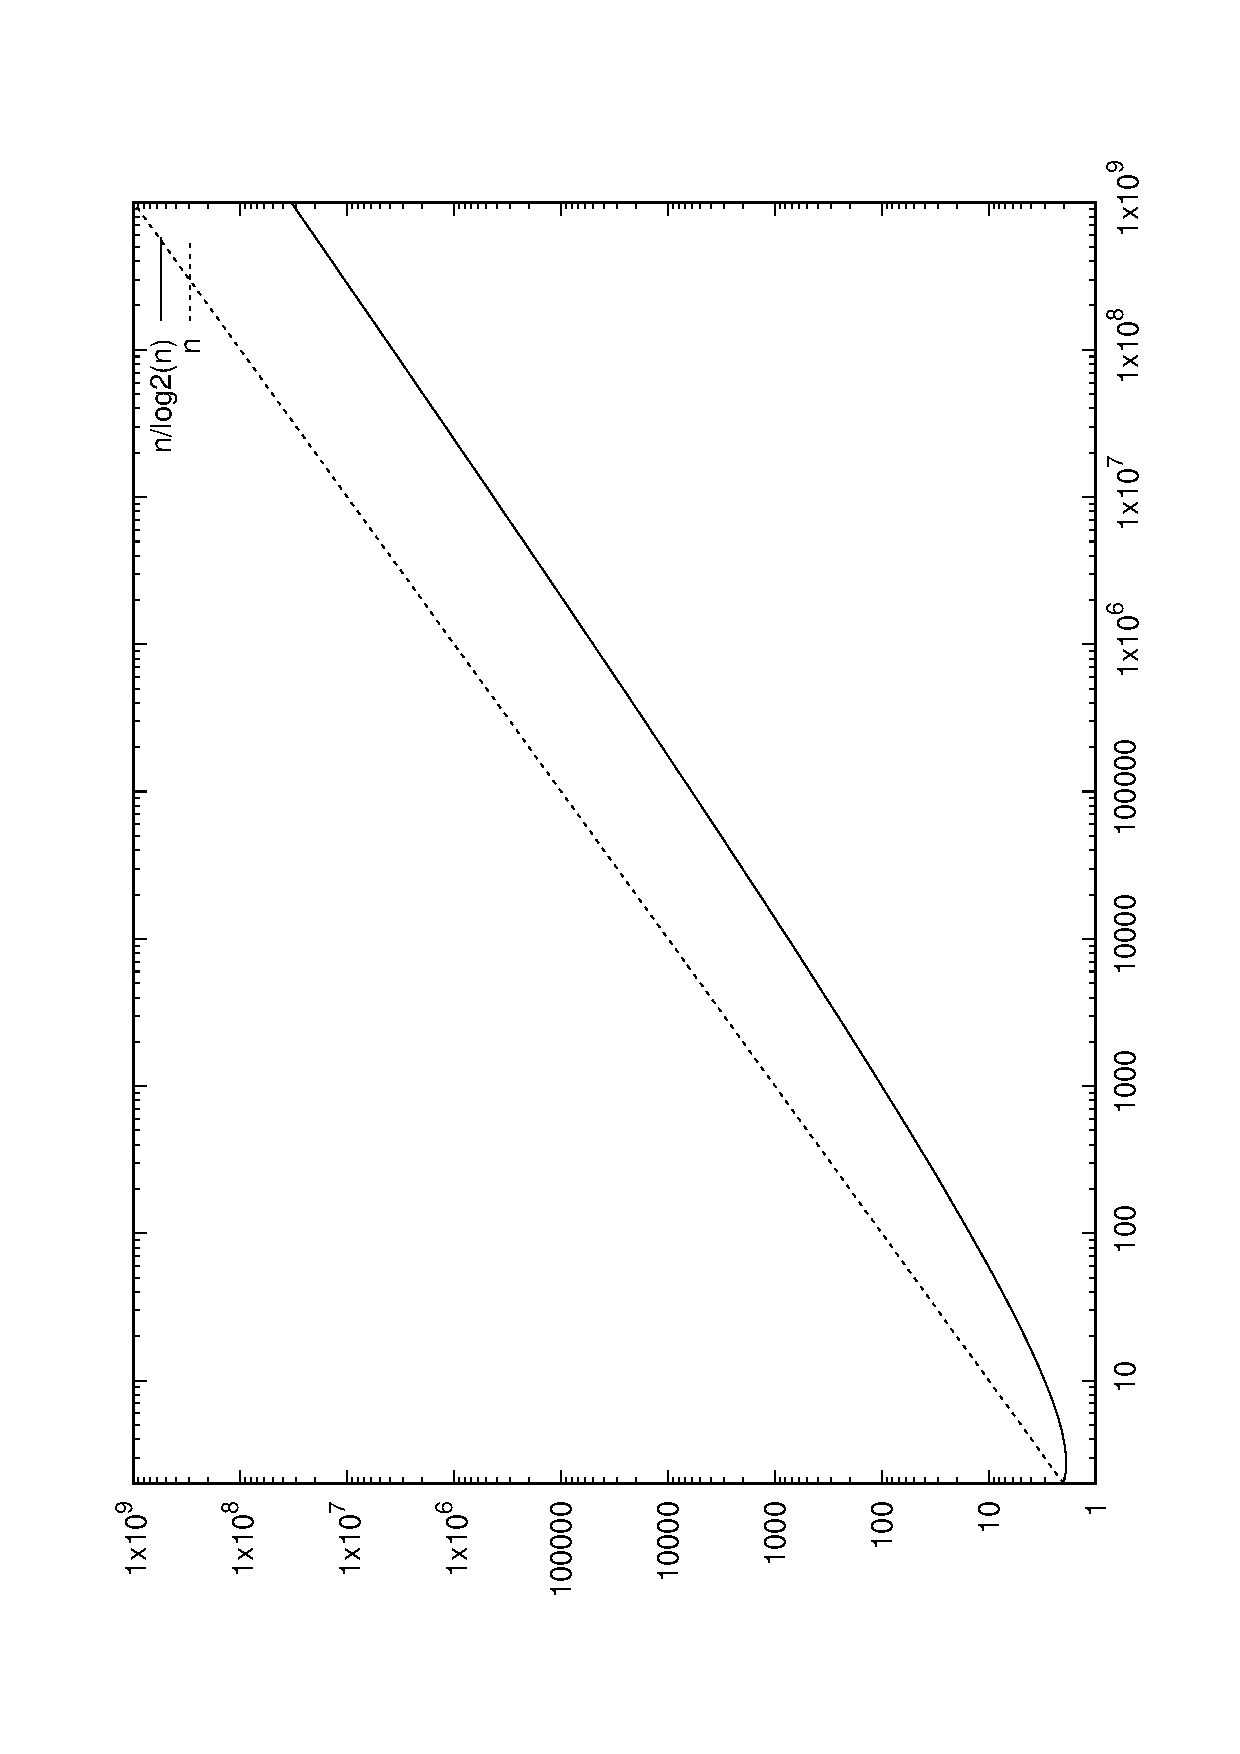
\includegraphics[width=.45\textwidth,angle=-90]{n-logn}}
    \end{center}
  \end{frame}

  \begin{frame}{Efficiency}
    \begin{block}{Efficiency ($E=S/p$)}
      \begin{itemize}
        \item the ratio of speedup to the number of processing elements --- the
          fraction of time for which a processing element is usefully employed
      \end{itemize}
    \end{block}
    \note[item] {Adding numbers --- $E=\theta(n/\log n)/n=1/\log n$}
    \note[item] {Matrix-vector --- $E=\theta(n)/n=1$}
    \note[item] {Matrix-matrix --- $E=\theta(n)/n=1$}
    \note[item] {Why do you think that the efficiency of adding numbers is less
      than matrix-vector or matrix-matrix?}
    \note[item] {What are the limits of efficiency?}

    \vspace{-2ex}
    \begin{center}
      \only<2>{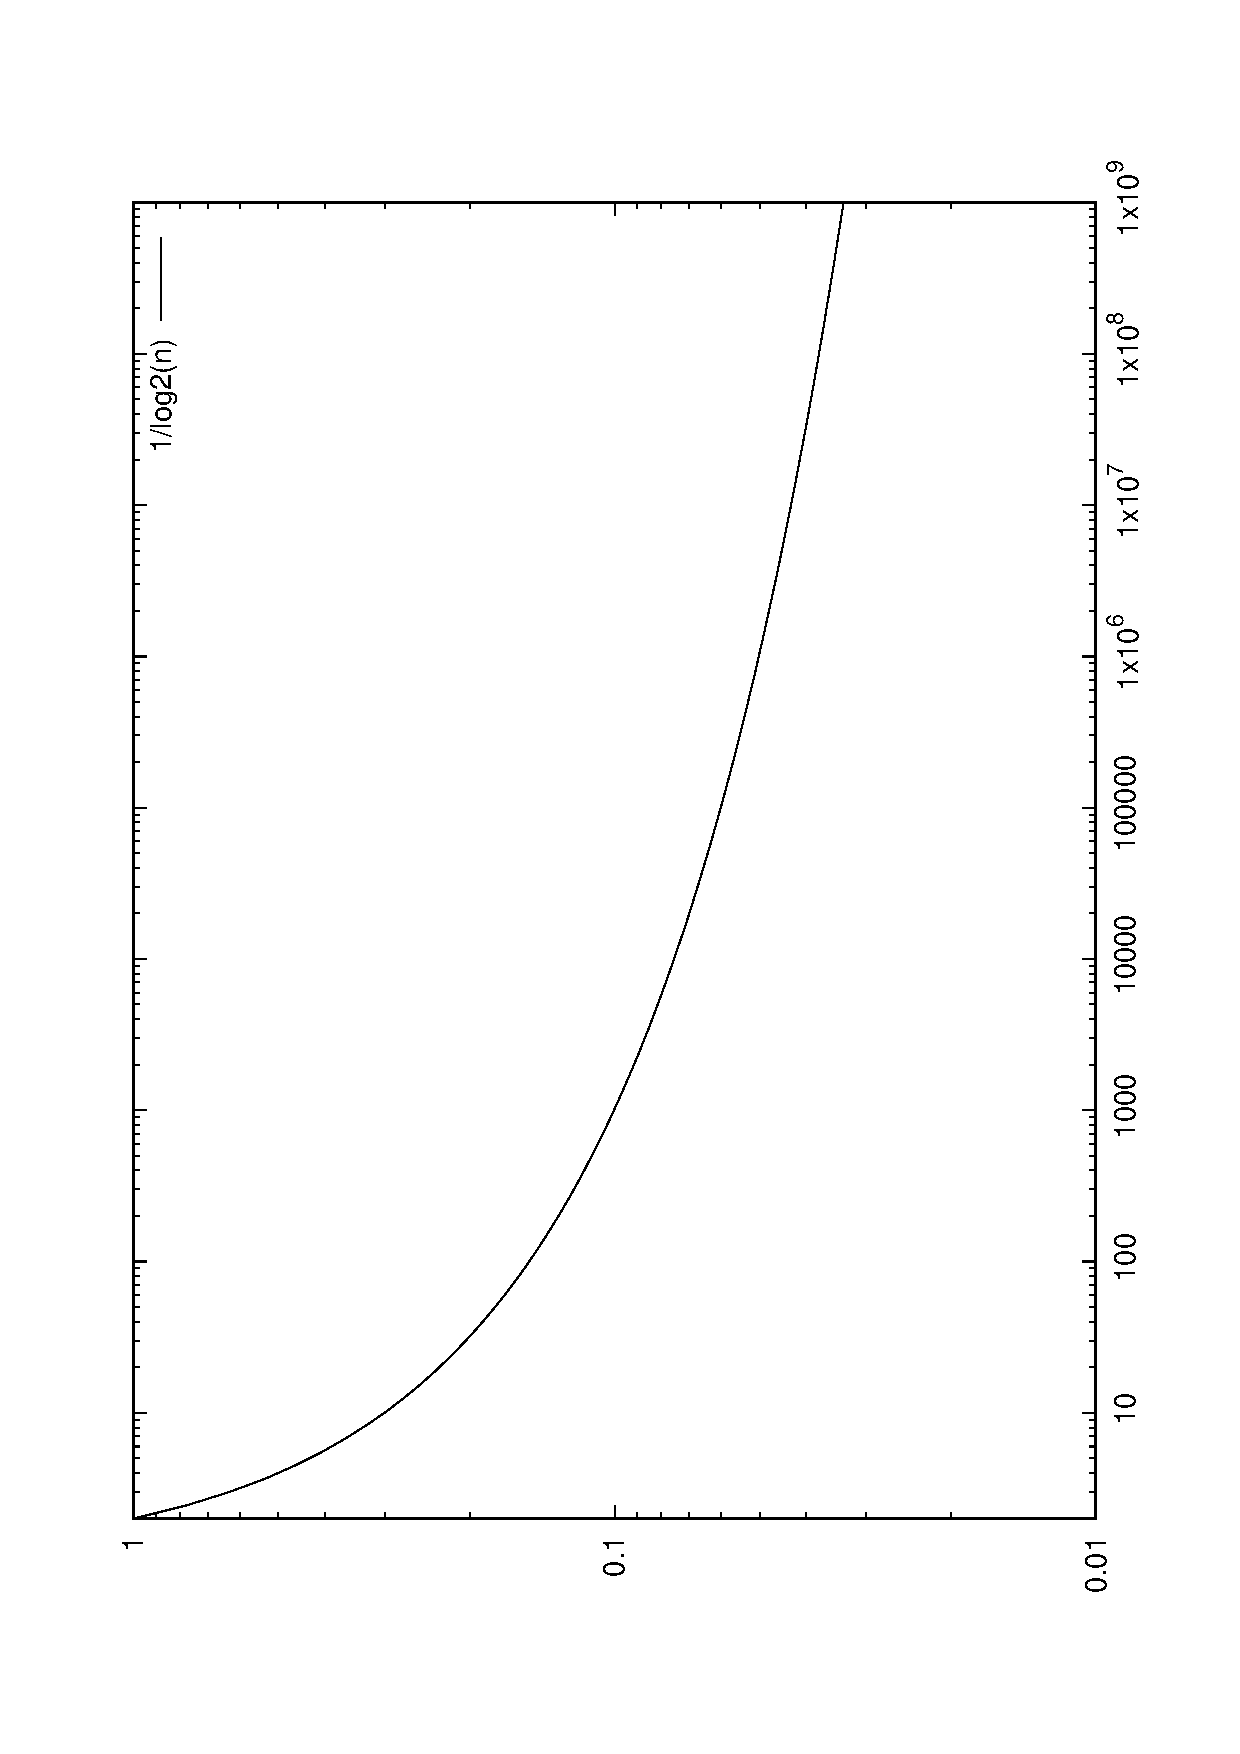
\includegraphics[width=.45\textwidth,angle=-90]{1-logn}}
    \end{center}
  \end{frame}

  \begin{frame}{Cost}
    \begin{block}{Cost ($C=pT_p$)}
      \begin{itemize}
        \item the sum of the time spent by all processing elements solving the
          problem
        \item \emph{cost optimal} if $C=T_s$
      \end{itemize}
    \end{block}
    \note[item] {Adding numbers --- $C=n\log n$}
    \note[item] {Matrix-vector --- $C=n\times n=n^2$}
    \note[item] {Matrix-matrix --- $C=n\times n^2=n^3$}
    \note[item] {Adding numbers is not cost optimal, the others are}

    \vspace{-2ex}
    \begin{center}
      \only<2>{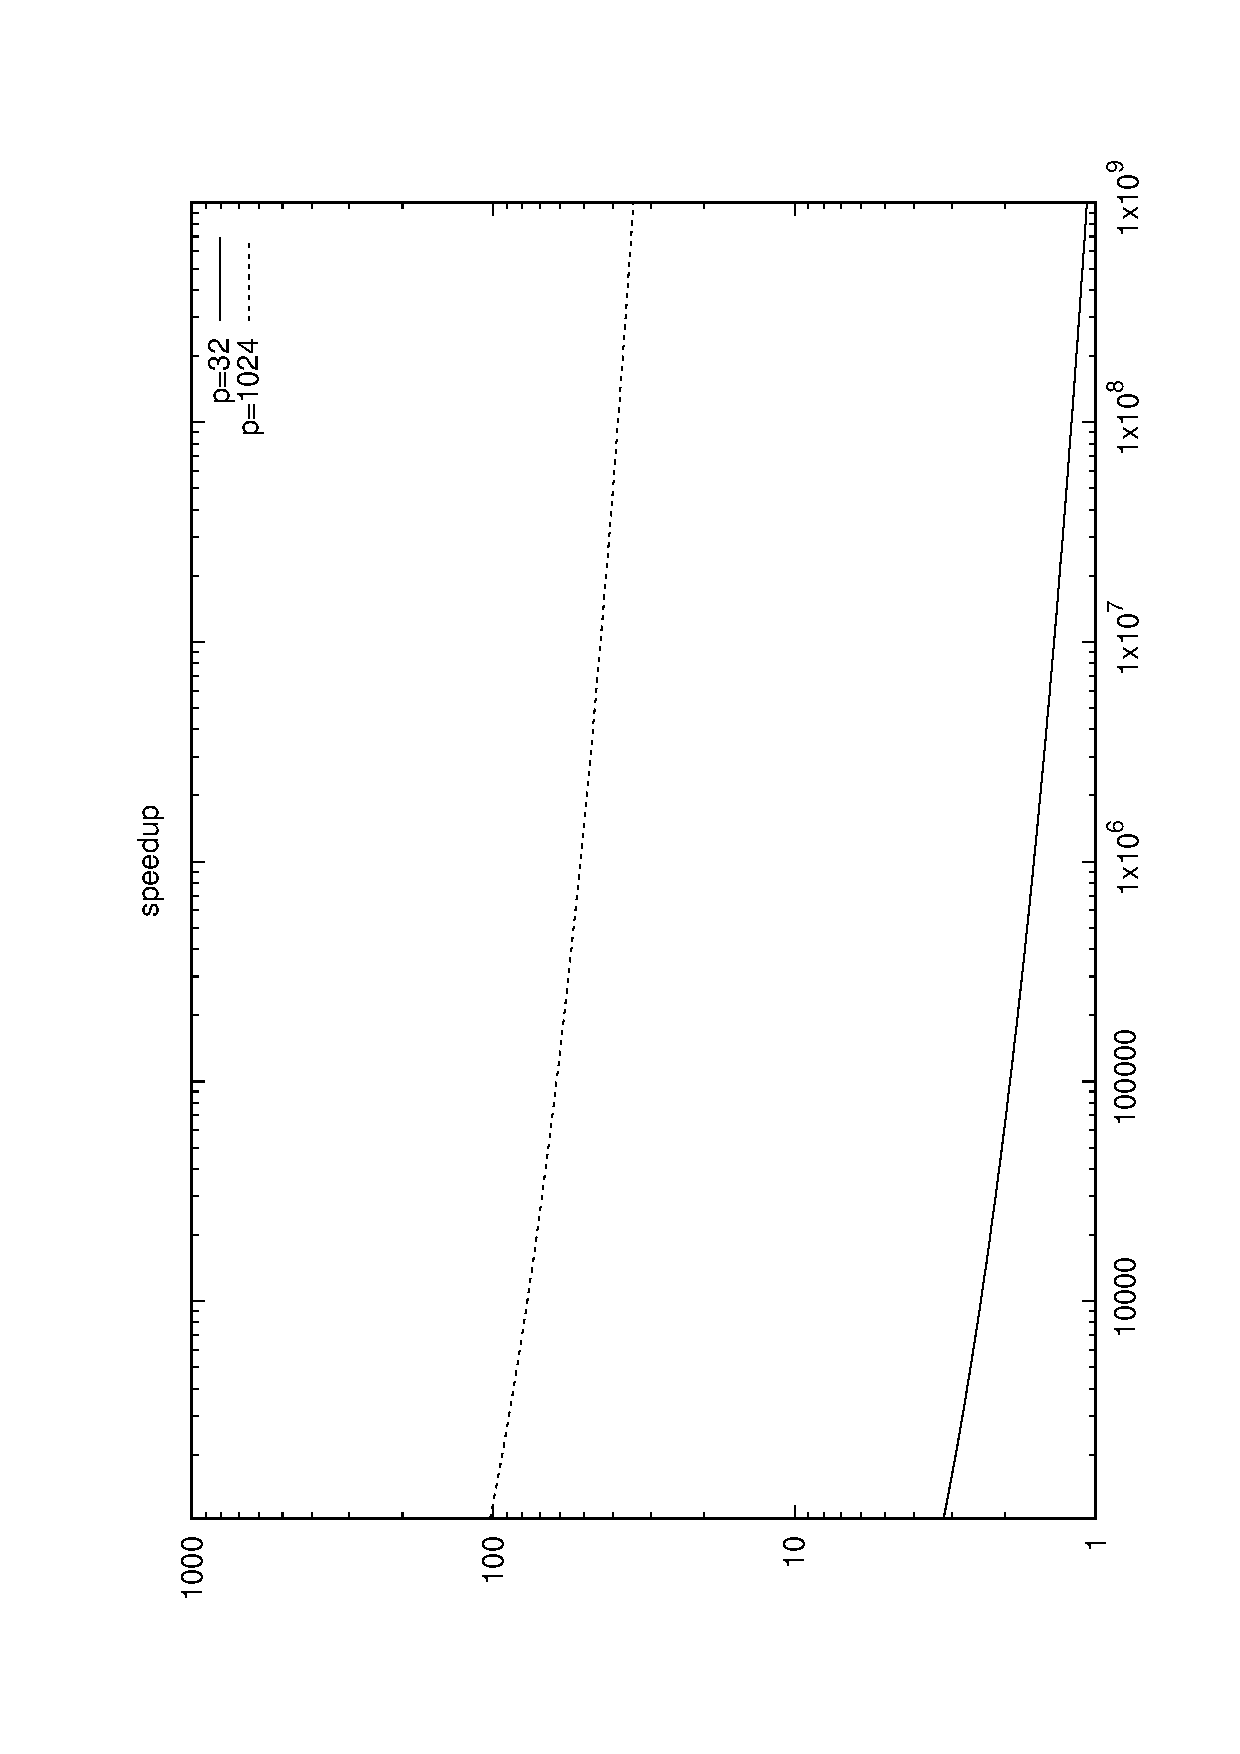
\includegraphics[width=.45\textwidth,angle=-90]{p-logn}}
    \end{center}
  \end{frame}


  %\begin{frame}[standout]
  %  \ifnotes
  %    \usebeamercolor[white]{normal text} % override bug fix in preamble
  %  \fi
  %\end{frame}

  \appendix

  \begin{frame}[c]
    \begin{center}\ccbysa\end{center}

    except where otherwise noted, this worked is licensed under
    \href{http://creativecommons.org/licenses/by-sa/4.0/}{creative commons
    attribution-sharealike 4.0 international license}
  \end{frame}
\end{document}
